\documentclass[openright,oneside,a4paper,english,12pt]{book}
\newcommand{\dir}{/Users/s0784966/Desktop/Test}

\usepackage{fancyhdr}% Use titlesec to put Chapter title on right
\usepackage{babel}
\usepackage{a4}
%\usepackage{sectsty}
\usepackage[round]{natbib}
\usepackage{amsfonts}
\usepackage{amsthm}
\usepackage{eucal}
\usepackage[intlimits]{amsmath}
\usepackage{epsfig}
\usepackage{graphicx}
\usepackage{lscape}
\usepackage{longtable}
\usepackage{rotating}
%\usepackage{supertabular}
%\usepackage{nomencl}
\usepackage[percent]{overpic}
%\usepackage{tocbibind}
\usepackage{caption}


%% some handy macros
\setlength{\headheight}{15pt}

\makeglossary
\newcommand{\pd}{\partial}
\renewcommand{\vec}{\boldsymbol}
\DeclareMathOperator{\Ber}{Ber}
\DeclareMathOperator{\Bei}{Bei}
\DeclareMathOperator{\Ker}{Ker}
\DeclareMathOperator{\Kei}{Kei}
\DeclareMathOperator{\integer}{int}
\DeclareMathOperator{\floor}{floor}
\DeclareMathOperator{\var}{var}
\DeclareMathOperator{\const}{constant}
\DeclareMathOperator{\maxval}{max}
%\bibliographystyle{plainnat}
\bibliographystyle{jmb}

% change font for captions
%\renewcommand{\captionfont}{\sffamily}
%\renewcommand{\captionlabelfont}{\bf}

% change font for chapter/section headings
%\allsectionsfont{\sffamily}

% funky graphics + text in lr bottom
\begingroup% 
\ifx\MakeISMBox\undefined%
\gdef\MakeISMBox#1#2#3{%
  \begin{overpic}[width=#1]{#2}%
    %\put(0,0){\includegraphics[width=#1]{#2}}%
    \put(98,2){\makebox(0,0)[br]{#3}}%
  \end{overpic}}%
\fi\endgroup%

% workaround for color in ed_thesis
\begingroup% 
\ifx\color\undefined%
\gdef\color[#1]#2{}%
\fi\endgroup%

% workaround for href in ed_thesis
\begingroup% 
\ifx\href\undefined%
\gdef\href#1#2{#2}%
\fi\endgroup%

% defining units for nomenclature packages
\newcommand{\nomunit}[1]{%
%  \renewcommand{\nomentryend}{\hspace*{\fill}[#1]}%
}

% Alternative style of head and foot
\pagestyle{fancy}% Used when using fancyhdr.sty
\renewcommand{\headrulewidth}{0.4pt}
\renewcommand{\footrulewidth}{0pt}
\renewcommand{\chaptermark}[1]{%
 \markboth{\MakeUppercase{%
 \chaptername} \ \thechapter.%
 \ #1}{}}
\renewcommand{\sectionmark}[1]{%
 \markright{ \ \thesection%
 \ #1}{}}

%\rhead{\thepage}
\fancyhead[LE,RO]{\thepage}
\fancyhead[LO]{\sl \leftmark}
\fancyhead[RE]{\sl \rightmark}
\fancyfoot{}

%Tidy up hyphenations as best as possible
\pretolerance = 600 % covers most paragraphs
\tolerance = 7000 % covers the nasty cases

%Tidy up hanging sentences as best as possible
\widowpenalty=10000

% To get the correct margins for the regulations for psglg1 and psglg3
\setlength{\oddsidemargin}{1.35cm} %margins set up for psglg1
\setlength{\evensidemargin}{-0.1cm}
\setlength{\topmargin}{0cm}
\setlength{\textwidth}{14.55cm}
\setlength{\textheight}{22.3cm}



%========================= ALTERATIONS ========================= 

%Paragraphs
\setlength{\parindent}{0em}
\setlength{\parskip}{\baselineskip}

%Alternative methods
%\lefthyphenmin=63
%\righthyphenmin=63
%\hyphenpenalty=10000
\makeatletter
\renewcommand{\frontmatter}{\cleardoublepage\@mainmatterfalse}
\renewcommand{\mainmatter}{\cleardoublepage\@mainmattertrue}
\makeatother
%\fancyhf{}
%\cfoot{\thepage}
%\pagestyle{fancy}     


\begin{document}

\frontmatter


\title{%
\textbf{Understanding how selection at linked sites influences patterns of genetic diversity in the house mouse} \\
	\large Or: What’s the deal with selective sweeps?}
\date{}

 
\maketitle

% Have Roman numeral for the frontispiece
\pagenumbering{roman} 

 
%\chapter{Acknowledgements}

First and foremost, thanks to Peter Keightley. He has been an excellent supervisor and mentor for the last four years. Peter's help and guidance has helped me develop in many ways and has made my PhD an incredibly enjoyable and rewarding experience. Peter's thorough and rigorous approach to science is something that I aspire to. Thanks for introducing me to disc golf too!

I would also thank Brian Charlesworth for helping me understand the thornier aspects of population genetics that I have come across. Brian has been very patient with me and willing to give help and advice whenever I have asked for it, which has been hugely helpful throughout my PhD.

Thanks to Deborah Charlesworth for being very kind and generous in helping me understand many aspects of evolutionary biology, not limited to my own research. Thanks to participants of the evolutionary genetics lab group and genetics journal club in IEB for great discussions and feedback about my research, particularly Susie Johnston and Konrad Lohse.

Thanks to members of the Keightley lab past and present for listening to me go on and on about selective sweeps or other things for the past four years. In no particular order: thanks Ben Jackson, Rory Craig, Susanne Kraemer, Eva Deinum, Thanasis Kousathanas and Matty Hartfield. Rob Ness taught me to code and helped me out in numerous ways, it's just a shame he left Edinburgh when he did. Without the help of Dan Halligan, who tolerated me bugging him even after he left the lab, I would have been very lost.

I would also extend massive thanks to Sally Otto and members of her lab group at UBC for giving me such a welcoming place to work and write-up my thesis in Vancouver.

On the personal side of things, thanks to my friends in IEB and the whole Berwickshire gang for palling around with me in Edinburgh. Thanks to Jaz and Michael for all the great hangs in Vancouver. 

My family has been very supportive throughout my whole PhD, particularly my amazing Mum and Dad. My brothers and their SAPs are great too, but Stella, you really nailed it.

Finally, Arya has looked after me and kept my head straight for the past four years. She is the best and even married me during this PhD, can you believe that?


\mainmatter
\renewcommand{\contentsname}{Table of Contents}
\tableofcontents

% Have arabic numerals for the actual meat
\pagenumbering{arabic} 

% Boot up the Chapter 1: Introduction file
\chapter{Introduction}
\chaptermark{Introduction}

\section{Understanding the causes of variation in genetic diversity}

	\textit{``If we take the Darwinian view that evolution is the conversion of variation between individuals into variation between populations and species in time and space, then an essential ingredient in the study of evolution is a study of the origin and dynamics of genetic variation within populations"}(Lewontin 1974)

\noindent
This quote, from Lewontin's 1974 book \textit{The Genetic Basis of Evolutionary Change}, eloquently demonstrates that understanding the causes of variation between and within populations is one the central goals of evolutionary genetics, and has been for a long time.
	
	 In the latter half of the $20^{th}$ century, one of the foundational theories in population genetics was developed, the neutral theory of molecular evolution. The neutral theory contended that molecular changes between populations were predominantly the result of random changes in allele frequencies through time \citep{RN175}. In the past 30 years of population genetic research, the increasing availability of DNA sequence data has led to an understanding that neutral evolution cannot readily explain patterns of variability and between within species \citep{RN358}. However, an understanding of the factors that shape molecular variability in natural populations is far from complete.

	In this thesis, I describe three projects in which I have analysed different aspects of population genomic data from wild mice. Each project aims to increase our understanding of the factors shaping molecular variation in the genome. Wild mice are an excellent model system for studying molecular evolution in mammals for several reasons. Firstly, being one of the most well-studied organisms in all of science, the genomic resources developed for \textit{Mus musculus} are among the best available for any animal. Secondly, the size of wild mouse populations are very large, which results in high levels of genetic diversity (\textit{see below}), increasing power to statistical analyses. 

\section[Core concepts]{Core concepts in evolutionary genetics}

	Throughout this thesis I will refer to a number of fundamental concepts in population genetics. I give a brief description of several of these here.

\subsection{Genetic drift}

	In a finite population, the random sampling of individuals contributing to the next generation causes stochastic changes in allele frequencies. In a randomly mating, diploid population with non-overlapping generations of size \textit{N}, the probability that a new mutation, free from the effects of selection, goes to eventual fixation is simply its starting frequency, $\frac{1}{2N}$ (assuming autosomal inheritance). This implies that for any new, neutral mutation that arises, there is much larger probability, $1 - \frac{1}{2N}$, that it will be lost from the population. The change in allele frequency caused by random sampling is termed genetic drift. Genetic drift is very effective in small populations and less effective in large populations. As populations tend to infinite size, allele frequencies are not, on average, expected to change from generation to generation.
	
	The idealised population described above is referred to as a Wright-Fisher population. Natural populations obviously violate the assumptions of a Wright-Fisher population, for example humans have overlapping generations. In the above statement of the probability of fixation in the Wright-Fisher model, the census number of individuals ($N$) appeared. In order to model genetic drift for populations that violate the assumptions of the Wright-Fisher model, the effective population size ($N_e$) is used. Note that there is often a discrepancy between $N_e$ and $N$, for example the population undergoes inbreeding, $N_e$ is reduced by $N$. Natural selection is less effective if $N_e < N$ than in a Wright-Fisher population of size $N$ (see below) \cite{RN110}.

	Genetic drift does not operate solely on neutral alleles, indeed advantageous alleles may be lost through random sampling, but the probability of this depends on the selection coefficient (\textit{see below}).
	
\subsection{Neutrality and coalescence}

	The neutral theory of molecular evolution, proposed by Motoo Kimura, and later refined with Tamoka Ohta (Kimura 1982), posited that the vast majority of molecular evolution could be attributed to genetic drift with only a minority attributable to adaptation. In the strict sense, the neutral theory deals with mutations that are completely free from selective effects. A more relaxed definition, referred to as the \textit{nearly} neutral theory includes mutations that are weakly deleterious, such that their fates are predominantly decided by drift (\textit{see below}). Although tenets of the neutral theory have largely been shown to not hold in natural populations ( Kreitman 1996, \citep{RN358, RN357}, the use of neutrality as a null hypothesis in molecular evolution has led to the development of a large number of statistical tests and the development of the coalescent.

	The coalescent is a framework for modelling molecular evolution that considers the evolutionary history of a sample of alleles drawn from a population. Working backwards in time, two alleles are said to \textit{coalesce} when they share a common ancestor at a particular time in the past. The probability of coalescence $t$ generations ago for a pair of neutrally evolving alleles is,
	\begin{equation}
	Pr(t) = \Big(1 - \frac{1}{2N}\Big)^{t-1}\frac{1}{2N}.
	\label{eq:coal}
	\end{equation}
\noindent
Equation \ref{eq:coal} is a geometric distribution, which, as $N \to \infty$ can be approximated by the continuous time exponential distribution. The rate parameter of this exponential distribution is $\lambda = \frac{1}{2N}$. Since the mean of the exponential distribution is the reciprocal of the rate parameter, the mean time to coalescence for a pair of randomly selected neutral alleles  when $N$ is large is simply $2N$.
		
\subsection{Population structure}

	The simplest population genetic models assume that the gametes that are sampled to produce progeny for the next generation behave like beans in a bag, where each bean has an equal probability of being sampled. Natural population do not necessarily behave like beanbags, however. Consider the case of an animal species that populates a long narrow range that stretches from North to South. Individuals at the top of the range, when seeking a mate, will be more likely to reproduce with an individual in their vicinity, rather than one from the South. Over time, this could lead to differences in allele frequencies along the North/South gradient. If one were to sequence individuals from across the range and perform a population genetic analysis on the resulting data that makes the assumption of a single randomly mating population, the differences in allele frequency due to the population structure could generate spurious results. The hypothetical example given above is relatively crude, true populations may be structured in very subtle (or in some cases not so subtle) ways that influence data analysis. Throughout this thesis, population structure is not analysed explicitly, but it is discussed as a potential confounding factor.

\subsection{Mutation and genetic diversity}

	Mutation is the ultimate source of all biodiversity. Mutation can be defined as a heritable change in an organism's genetic sequence. Mutations may occur during DNA repair, be affected by physical or chemical agents (e.g. UV radiation) or caused by errors in replication during meiosis or mitosis. There are numerous categories of mutations that have been described (e.g. translocations, inversions, insertions, deletions and point mutations). The most common of type of mutations, and the one most pertinent to this thesis, is single nucleotide substitution or point mutation. Point mutations involve the change of a single nucleotide from one of the four bases to another (e.g. adenine to cytosine). The rate of point mutation is higher than for small insertions and deletions, perhaps as much as an order of magnitude higher than for small insertion and deletions (Keightley et al. 2013). Throughout this thesis I deal only with point mutations, unless otherwise stated.

	Depending on the population size, new mutations may be heavily influenced by genetic drift. The rate at which new mutations enter into the population obviously depends on population size, the more individuals there are, the more chances there are for mutations to occur. The probability that two randomly chosen individuals differ at a particular nucleotide in the genome depends on the time since they shared a common ancestor $t$. Working backwards along the two branches leading to the common ancestor, there is a total of $2t$ generations separating the two alleles. If the per site per generation mutation rate is $\mu$, then in the time separating two alleles, there is a probability of $2t$ that a mutation arose. As we saw above, the mean time to coalescence for pair of neutral alleles is $2N_e$, so the probability that two randomly chosen alleles differ is
	\begin{equation}
	\theta = 4N_e\mu. 		
	\end{equation}
\noindent
The average number of pair wise differences between sequences ($\pi$) therefore gives an estimate of the probability that two randomly chosen alleles differ in state, so $\pi$ can be used as an estimator of $\theta$. This quantity, $\pi$, or $\theta_{\pi}$ as it is sometimes denoted, is easily calculable from the polymorphism data. 


\subsection{Selection}

	The vast majority of the mouse genomes is not evolutionarily conserved, and thus can be inferred to be non-functional \citep{RN161}. Most mutations that occur will, therefore, not affect  their carriers' fitness. However, new mutations occurring in functional regions may be subject to selection. Throughout this thesis, I will refer to the selection coefficient ($s$), which is defined in terms of the relative fitnesses of the three genotypes possible at a biallelic locus, where $A$ is the wild-type allele and $a$ is the allele subject to selection:

\begin{center}
\begin{tabular}{c | c | c | c }
	Genotype & AA & Aa & aa \\ \hline
	Fitnesses& $1$ & $1 + sh$ & $1 + s$ \\
\end{tabular}
\end{center}	

\noindent

Here, $h$ is the dominance coefficient of new mutations; under additivity $h = 0.5$,  complete dominance $h = 1$, complete recessivity $h = 0$, and heterozygote advantage $h > 1$. In this thesis, selected mutations are assumed to behave additively, unless otherwise stated. 

	Even when selection is acting on a new mutation, genetic drift may still operate. As derived by both Kimura (1962) and Fisher (1930), the fixation probability for a semi-dominant mutation with selective effect $s$, segregating at a frequency of ($q$) in a population of size $N_e$ is,

\begin{equation}
	u(s, N_e, q) = \frac{1 - e^{-2N_esq}}{1 - e^{-2N_es}}
	\label{eq:fixation}
\end{equation}

\noindent
In a Wright-Fisher population, the frequency of a new mutation is $\frac{1}{2N}$, so the exponent in the left-hand side of the numerator in Equation \ref{eq:fixation} is $\approx s$. From Equation \ref{eq:fixation}, it can be observed that the fixation probability of a new mutation is dependant on the relative magnitude of $N_e$ and $s$. If $N_e$ were large and the mutation were advantageous, the denominator $(1 - e^{-2N_es}) \to 1$, so $u(s, N_e, q) \approx s$. If the product $N_es \gg 1$, then the mutation behaves deterministically. In the case of deleterious mutations, (where $s < 0$), if $|N_es| > 1$ then $u(s, N_e, q) \to 0$.  For both advantageous and deleterious mutations if $|N_es| \leq 1$, then the fate of the mutation is similar to that of a neutral allele and genetic drift dominates. The factors that can affect $N_e$ (e.g. inbreeding, sex structure and popualtion strucure) cause a reduction in the efficacy of selection. If the effective population size, $N_e$, fell below the census size, $N$, then the fixation probabilities for strongly beneficial mutations will be reduced by a factor $N_e/N$.

	Throughout this thesis I frequently use the term neutral to describe molecular evolution dominated by genetic drift, including cases where $s << \frac{1}{2N_e}$

\subsection{The McDonald-Kreitman test}

	One of the most widely used methods for the detection of positive selection is the McDonald-Kreitman (MK) test \citep{RN293}. The MK-test contrasts molecular variation at putatively neutral sites with variation at potentially selected sites. Typically, synonymous and nonsynonymous sites in protein-coding genes are used as the neutral and selected site categories, respectively. Under the neutral theory, differences between species accumulate by the random fixation of neutral  alleles due to drift, with a negligible contribution from positive selection. As such, the ratio of nucleotide diversity at nonsynonymous/synonymous sites ($\pi_N / \pi_S$) should be statistically indistinguishable from the ratio of nonsynonymous/synonymous divergence ($d_N / d_S$). An elevation of $d_N / d_S$ above the value expected given $\pi_N / \pi_S$ is taken as evidence for positive selection. The MK-framework has been expanded to allow the estimation of the proportion of nucleotide substitutions at a particular class of sites, driven by positive selection ($\alpha$)

\begin{equation}
\alpha = 1 - \frac{d_N \pi_N}{d_S \pi_S}.
\end{equation}

\citep{RN294}. However, since weakly deleterious mutations at, for example, nonsynonymous sites may segregate in a population, estimates of $\alpha$ obtained in this way are likely underestimates. Further developments of the MK-test have been made that estimate the distribution of fitness effects for new mutations and use this to correct for the contribution deleterious mutations make to both standing variation and between-species divergence when performing MK-type analyses \citep{RN165}. 

\subsection{Recombination}

	Recombination is a fundamental process in the evolution of sexual organisms. Recombination involves the transfer of information from one chromosome copy to another via crossing over, the reciprocal exchange, or swapping, of DNA between homologous chromosomes, or gene conversion, where there is a non-reciprocal exchange between homologous chromosomes. In mammals, recombination is integral to the successful segregation of chromatids during meiosis. If recombination is suppressed, there are far higher rates of aneuploidy and other meiotic errors (de Massey 2011). During meiotic prophase, after the pairing of homologous chromosomes, a series of double-strand breaks (DSBs) are formed in each of the four chromatids (de Massey 2011). DSBs are typically resolved in two ways, one that predominantly leads to crossovers and one that leads to gene conversions. In mice, PRDM9 is a zinc-finger DNA-binding enzyme that recruits the protein complex that initiates DSBs (de Massey 2011). In many organisms crossing-over events typically occur in narrow genomic windows, referred to as recombination hotspots, and in mice these are enriched for the bindings motifs of PRDM9 (de Massey 2011).

	Recombination is an important process in evolution and is thought to provide a substantial benefit to sexual reproduction. There are numerous theories as to why meiotic recombination evolved, which can be summarised as a) preventing selective interference, resulting in more efficient responses to selection b) providing a moving evolutionary target to parasites by generating new genotype combinations and c) breaking apart harmful combinations of alleles (Hartfield and Keightley 2012). Genetically linked sites do not evolve independently, selection acting at one may have consequences for another. Because of this, the rate of recombination influences the consequences of natural selection.

\section[Models of selective sweeps]{Models of selective sweeps}

\cite{RN124} showed that an advantageous mutation drags with it linked neutral polymorphisms as it rises in frequency. With increasing genetic distance from the selected site, the effect is reduced, resulting in troughs in genetic diversity in surrounding regions.
 
 \begin{figure}[h!]
   \centering      
   \noindent\makebox[\textwidth]{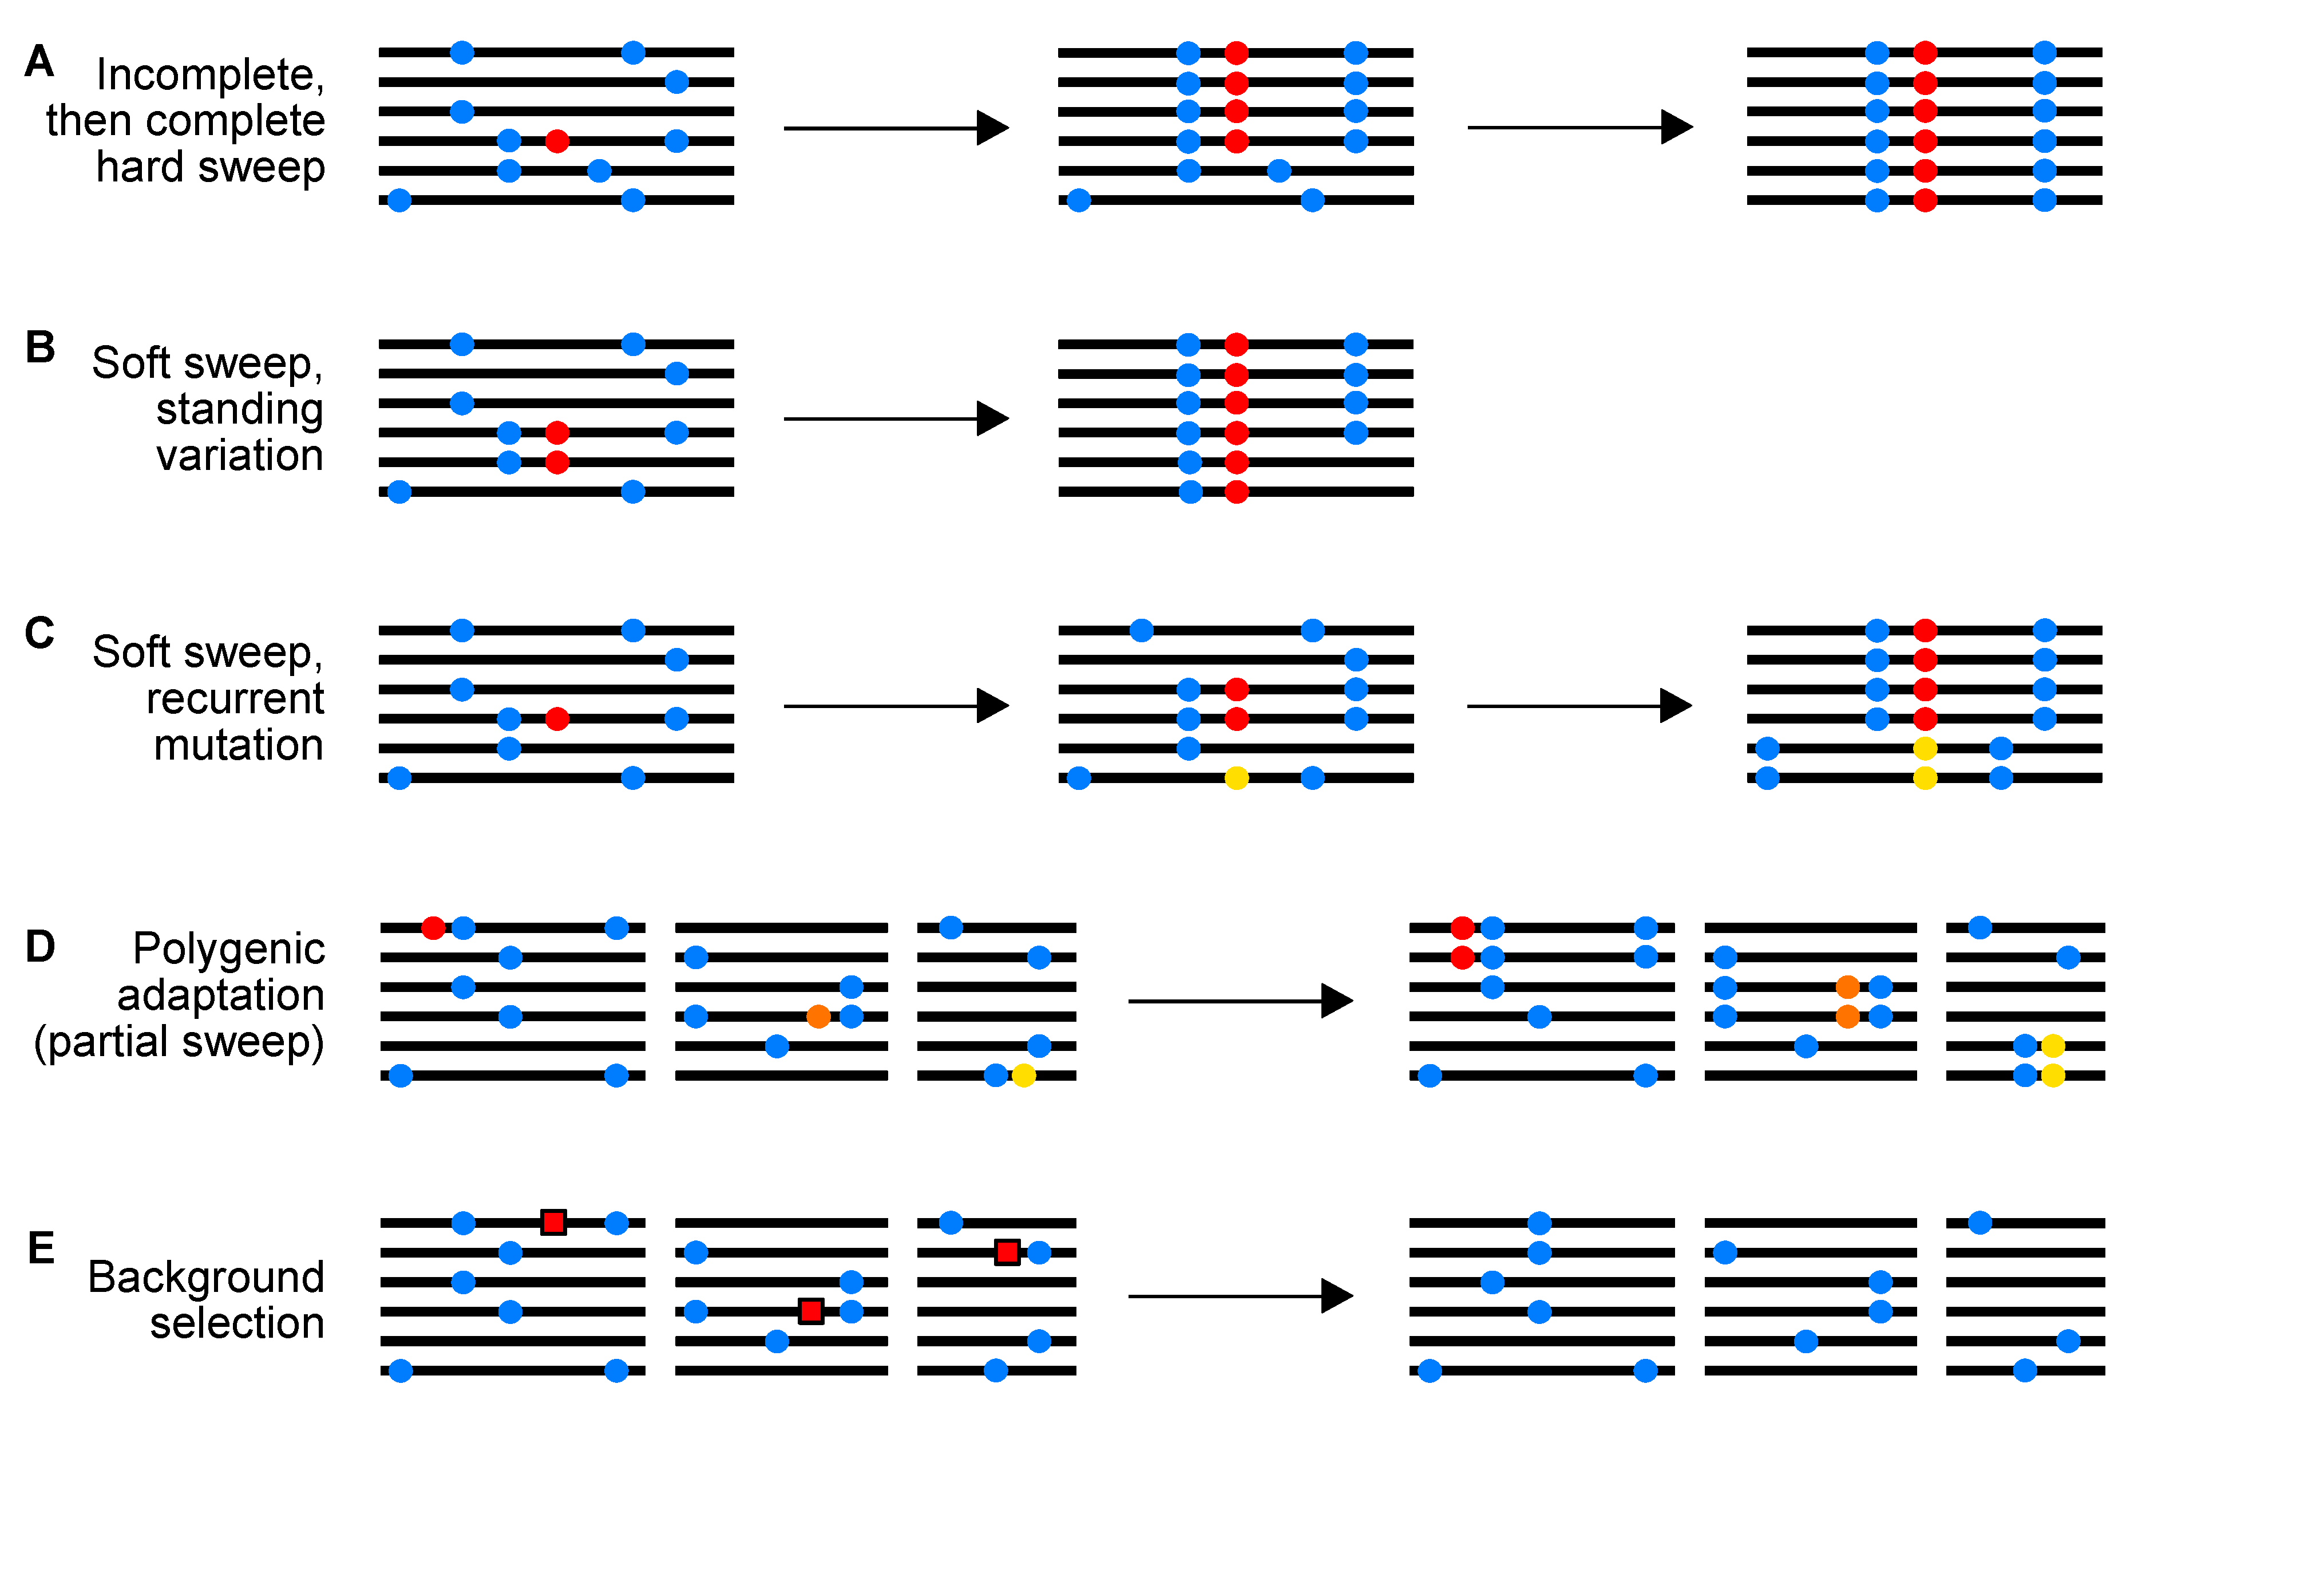
\includegraphics[width=\textwidth]{/Users/s0784966/Dropbox/Thesis/chapter1/figure_sweeps_no_legend.pdf}}
 \caption[Selective sweeps and background selection]{Selective sweeps and background selection. Blue circles represent neutral alleles, red, yellow and orange circles represent advantageous alleles, and red squares represent deleterious alleles. Reproduced from \cite{RN352}, courtesy of Ben Jackson.}.
 
 \label{fig:sweepCartoon}
\end{figure}


\subsubsection{Hard/classic sweeps} 
 
The most well-studied model of sweeps. A new advantageous mutation rapidly increases in frequency to eventual fixation (shown in Figure \ref{fig:sweepCartoon}-A). As it sweeps, the adaptive allele carries with it a portion of the haplotype on which it arose, reducing levels of neutral diversity in the surrounding area \citep{RN124,RN235}. 
 
\subsubsection{Soft sweeps} 
  
A neutral allele segregating in a population may become favoured (due, for example, to a change in the environment). The segregating allele may be associated with multiple haplotypes, and as it rises in frequency, so do the multiple haplotypes (shown in \ref{fig:sweepCartoon}-B). A similar process, also termed a soft sweep, can occur if an advantageous mutation arises by multiple, distinct mutation events (shown in \ref{fig:sweepCartoon}-C). 
 
\subsubsection{Incomplete/partial sweeps} 
 
If an advantageous allele increases in frequency, but does not reach fixation, there will still be some loss of linked neutral diversity. In this review we use the term incomplete sweeps to describe sweeps that are polymorphic at the time of sampling, but may (or may not) eventually reach fixation (shown in \ref{fig:sweepCartoon}-A). The term partial sweep describes the situation wherein a sweeping allele becomes effectively neutral at a certain frequency in its trajectory (shown in \ref{fig:sweepCartoon}-D). The magnitude of both processes on linked neutral diversity depend on the frequency reached by the sweeping allele when selection is ‘turned off’ or on the time of sampling \citep{RN226}. Partial sweeps may be common in cases of adaptation involving selection on quantitative traits \citep{RN147}. 

\subsection{Background selection} 
As natural selection purges deleterious mutations, neutral alleles linked to the selected locus are also lost. The process of background selection is qualitatively similar to recurrent selective sweeps, since both processes reduce local genetic diversity \citep{RN110} and skew the site frequency spectrum towards rare variants \citep{RN287, RN113}. Models of background selection envisage a neutral site linked to many functional sites at different distances, such that the effects of selection at many sites accumulate to reduce diversity \citep{RN206,RN157}. 

\section[Using models of selective sweeps to estimate positive selection parameters]{Using models of selective sweeps to estimate positive selection parameters}
 
Population geneticists have long sought to understand the contribution of natural selection to molecular evolution. A variety of approaches have been proposed that use population genetic theory to quantify the rate and strength of positive selection acting in a species’ genome. In the following section, I discuss methods that use patterns of between-species nucleotide divergence and within-species diversity to estimate positive selection parameters from population genomic data. We also discuss recently proposed methods to detect positive selection from a population’s haplotype structure. The application of these tests has resulted in the detection of pervasive adaptive molecular evolution in multiple species.
 
If adaptive substitutions are common, selection is expected to leave footprints in genetic diversity at linked sites. In particular, as a positively selected mutation increases in frequency, it tends to reduce diversity at linked neutral loci. Theoretical analysis of this process, termed a selective sweep (\textit{see above}), has shown that the reduction in diversity at a linked neutral locus depends on the ratio of the strength of positive selection to the recombination rate. Thus, comparing diversity at multiple neutral loci linked to selected regions, in principle, should provide an indirect means for estimating parameters of positive selection.

If a population experiences recurrent selective sweeps, there are several patterns predicted by theory. Under recurrent hard selective sweeps, levels of genetic diversity are expected to be lower i) in regions of the genome with restricted recombination, ii) in regions experiencing many sweeps and iii) in the genomic regions surrounding the targets of selection themselves. Each of these of these predictions have been met in empirical studies, and each has been used to estimate parameters of positive selection.

\subsection[The correlation between diversity and the rate of recombination]{The correlation between diversity and the rate of recombination}

In the late 1980s, evidence began to emerge suggesting that genetic polymorphism are less frequent in genomic regions experiencing restricted crossing-over \citep{RN225,RN282}. Soon after, \cite{RN114} showed that there is a positive correlation between nucleotide diversity and the rate of crossing-over in \emph{D. melanogaster}, a pattern subsequently observed in other eukaryotic species \citep{RN117}. Begun and Aquadro pointed out that the correlation is qualitatively consistent with the action of recurrent selective sweeps. \cite{RN277} formulated expressions, based on the correlation between nucleotide diversity and the rate of recombination, to estimate the compound parameter $\lambda 2N_{e}s$, where $\lambda$ is the rate of sweeps per base pair per generation, $N_e$ is the effective population size and $s$ is the selection coefficient. They applied their method to the data of \cite{RN114}, estimating $\lambda2N_{e}s$ = 5.37 x $10^{-8}$, but their method could not disentangle the individual parameters. More recently, \cite{RN226} performed a similar analysis in \emph{D. melanogaster} to explore the effects of partial sweeps on parameter estimates. They showed that when partial sweeps are common, the rate of adaptive evolution is underestimated if the hard sweep model is assumed.
 
The correlation between diversity recombination observed by \cite{RN114} can also be explained by background selection, the reduction in neutral diversity caused by the removal of linked deleterious mutations \citep{RN132}. The process of background selection is qualitatively similar to recurrent selective sweeps, since both processes reduce local genetic diversity \citep{RN110} and skew the SFS towards rare variants \citep{RN287,RN133}. Models of background selection envisage a neutral site linked to many functional sites at different distances, such that the effects of selection accumulate to reduce diversity \citep{RN206, RN157}. The correlation between neutral diversity and the recombination rate predicted by background selection is quantitatively similar to that observed in \emph{D. melanogaster} \citep{RN281}. Indeed, recent studies suggest that background selection is a major determinant of nucleotide diversity variation at broad scales ($>$100Kbp) in humans \cite{RN120} and \emph{D. melanogaster} \citep{RN288, RN116}. It is clear, then, that background selection is a key confounding factor when attempting to make inferences about positive selection.
 
\subsection[Correlations between neutral diversity and non-neutral divergence]{Correlation between neutral diversity and non-neutral divergence}

If there is a constant fraction of adaptive substitutions, $\alpha$, across the genome for a given class of sites, regions that evolve at higher rates should experience a greater number of selective sweeps. Under a model of recurrent sweeps, it follows that there should be a negative correlation between nucleotide divergence at selected sites and diversity at linked neutral sites. This was first described in \textit{Drosophila melanogaster} by \cite{RN283}, and has been subsequently reported in other \textit{Drosophila} species \citep{RN284}. Assuming a single rate of sweeps ($\lambda$) and a constant scaled strength of positive selection ($2N_es$) for a given class of sites, \cite{RN283} generalised formulae of \cite{RN277} based on the correlation between synonymous site diversity and non-synonymous site divergence to estimate  $\lambda 2N_es$ = $3 \times 10^{-8}$ for the X-chromosome in \textit{D. melanogaster}. Note that this $\lambda 2N_es$ estimate is similar to that obtained based on the correlation of synonymous site diversity and recombination rate (\cite*{RN277}; see above). Using an estimate of $\alpha = 0.50$ obtained from a MK-based analysis, \cite{RN283} decomposed the $\lambda 2N_es$ compound parameter, and inferred that $s \approx 0.001\%$ and $\lambda$ = $3.6 x 10^{-11}$ /bp/generation, suggesting that adaptation of protein-coding genes in \textit{D. melanogaster} is driven by moderately weak selection (i.e., assuming \textit{D. melanogaster} $N_e =10^6$, $2N_es \approx 40$). In a related study, \cite{RN289} estimated $\lambda 2N_es \approx 10^{-7}$ in \textit{D. simulans}, also by examining the correlation between mean neutral diversity and selected (nonsynonymous) divergence. However, their model also included the heterogeneity in levels of diversity, which is related to the rate and strength of sweeps in a different way to the mean, and allowed the individual parameters to be fitted by regression. The estimates of the compound parameter $\lambda 2N_es$ are similar between the two studies, though \cite{RN289} estimated that $s \approx 1\%$ (compared to Andolfatto’s estimate of $s \approx 0.001 \%$) and $\lambda = 3.6 \times 10^{-12}$ /bp/generation. The discrepancies between the studies may be due to differences in biology between the species, or may reflect methodological differences: For example, if the majority of adaptive substitutions are driven by weakly selected sweeps, which will leave a relatively small signal in levels of  polymorphism, the MK-based method may more sensitively detect them, perhaps explaining the higher rate of sweeps inferred by \cite{RN283}. On the other hand, strongly selected sweeps will leave a larger footprint in levels of diversity, so will be more readily detected using the approach of \cite{RN289}, perhaps explaining why they inferred a lower overall rate of sweeps, with higher selection coefficients (for a full description, see \citealt{RN171}). In both cases, inferences based on variation in polymorphism may reflect processes other than the fixation of adaptive alleles that have gone to fixation, such as partial sweeps and background selection, as these will affect patterns of diversity but not necessarily divergence. Related to this, the approach employed by \cite{RN283} has recently been extended by \cite{RN323}, by estimating the correlation between synonymous site diversity and non-synonymous divergence in the presence of both background selection and gene conversion in \textit{D. melanogaster}. They found that ignoring background selection tends to increase and decrease estimates of selection strength and rate, respectively. The parameter values estimated in their study suggest that 0.02\% of new mutations at nonsynonymous sites are strongly selected ($s \approx 0.03\%$, assuming $N_e$ = $10^6$ for \textit{D. melanogaster}).
 
\subsection[Patterns of diversity around the targets of selection]{Patterns of diversity around the targets of selection}
 
An individual hard selective sweep is expected to leave a trough in genetic diversity around the selected site. If a large proportion of amino acid substitutions are adaptive, as suggested by MK-type analyses (see \citealt{RN215}), collating patterns of diversity around all substitutions of a given type should reveal a trough in diversity. Such a pattern is not expected around a “control” class of sites, such as synonymous sites. This test, proposed by \cite{RN167}, was first applied it to \textit{D. simulans}, and the above pattern was found. By fitting a hard sweeps model to the shape of the diversity trough, they estimated α values of  5\% and 13\%, depending on whether one or two classes of beneficial mutational effects were fitted. Note that their estimates of α are substantially lower than those obtained using MK-based methods for \textit{D. melanogaster} \citealt{RN283}. \cite{RN167} suggested that modes of selection other than hard sweeps may help explain to this discrepancy. However, even when modelling two classes of beneficial mutations, they found that amino acid substitutions are driven by strongly adaptive mutations ($s$ $sim0.5\%$ and $s$ $\sim0.01\%$). Their estimates of selection strength are therefore in broad agreement with the estimate of s $sim1\%$ obtained by \cite{RN289}, based on the correlation between synonymous diversity and non-synonymous divergence in \textit{D. simulans}. The \cite{RN167} test, then, suggests that adaptation in protein-coding genes is fairly frequent and driven by strong, hard sweeps.
 
The Sattath test has been applied in a variety of organisms, including humans \citep{RN162}, wild mice \citep{RN122}, \textit{Capsella grandiflora} \citep{RN236} and maize \citep{RN230}. In all but \textit{C. grandiflora}, researchers have found no difference in patterns of diversity around selected and neutral substitutions. These results have been interpreted as evidence that hard sweeps were rare in the recent history of both humans \citep{RN162} and maize \citep{RN230}. However, \cite{RN237} pointed out that the Sattath test will be underpowered if there is large variation in levels of functional constraint in the genome. Indeed, through their analyses \cite{RN237} found evidence for frequent adaptive substitutions in humans, particularly in regulatory sequence. To address the issues raised by \cite{RN237}, \cite{RN230} applied the Sattath test to substitutions in maize genes with the highest and lowest levels of functional constraint separately, but still found no difference in diversity pattern, suggesting either that hard sweeps have been rare in that species or that there is another confounding factor.
 
One possible explanation is that the species in which the Sattath test did/did not detect hard sweeps have distinct patterns of linkage disequilibrium (LD). LD decays to background levels within hundreds of base-pairs in \textit{D. simulans} \citep{RN283} and \textit{C. grandiflora} \citep{RN271}, whereas in humans, maize and wild mice it decays over distances closer to 10,000bp \citep{RN273,RN327, RN272}. It may be, then, that the Sattath test is only applicable when there is relatively short-range LD, such that the patterns of diversity around selected substitutions do not substantially overlap with the analysis windows around neutral ones. If this were the case, interpreting the similarity in troughs of diversity around selected and neutral substitutions as evidence for a paucity of hard selective sweeps may not be justified in organisms where LD decays over distances of a similar order of magnitude as the width of the diversity troughs themselves.
   	        	  
\section[Fitting genome wide patterns]{Fitting genome wide patterns}

	Methods to estimate the rate and strength of positive selection in the genome employ various combinations of nucleotide diversity, divergence, recombination rates and estimates of background selection effects as summary statistics, averaged over many regions of the genome. Recently, \cite{RN274} developed a method that fits a model of hard sweeps and background selection to genome-wide variation in nucleotide diversity and divergence (at both selected and neutral sites). In \textit{D. melanogaster}, they showed that hard sweeps can explain a large amount of genome-wide variation genetic diversity. For nonsynonymous sites, they found that $\alpha = 4.1\%$ for strongly selected mutations ($s \geq 0.03\%$) and $\alpha = 36.3\%$ for weakly selected mutations ($s \approx 0.0003\%$), summing to $\alpha = 40.4\%$, which is similar to the estimate obtained using the MK-test \citep{RN283}. Their results suggest that accounting for weakly selected mutations may help reconcile the discrepancy between MK-based estimates of the rate and strength of selection and parameters estimated from sweep model predictions, described above.

\cite{RN274} showed that a map of the effects of hard sweeps and background selection is capable of explaining a large amount of the variation in diversity across the genome, further demonstrating that the action of natural selection is pervasive, at least in \textit{D. melanogaster}. However, their method overestimated the rate of deleterious mutations, which the authors attribute to the presence of modes of adaptation other than hard sweeps in \textit{D. melanogaster}. 

\section[\cite{RN122}]{\cite{RN122}}


	The research I have performed throughout my PhD carries on from the work of \cite{RN122}, it is fitting, therefore, to give a brief description of the key findings from that study.
	
	\cite{RN122} sequenced the genomes of 10 wild-caught \textit{Mus musculus castaneus} individuals, using high-throughput sequencing methods. They sequenced individuals to high coverage, using multiple libraries of Illumina paired-end reads. Based on an analysis of population structure, the individuals sequenced were thought to represent a single admixed group. \cite{RN122} extracted polymorphism data from genomic regions surrounding both protein-coding exons and conserved non-coding elements (CNEs - which were inferred to be involved in gene regulation), and found dips (or troughs) in average diversity surrounding the elements themselves. As discussed above, \cite{RN122} applied the Sattath analysis to their data, but found that there was no difference in the average diversity around nonsynonymous/synonymous substitutions. They also modelled the contribution BGS made to the troughs in diversity around both protein-coding exons and CNEs using a population genetic model, and found that it could not fully explain the observed patterns of diversity. Our understanding of the factors that shape nucleotide diversity across the mouse genome are, thus, somewhat unclear.

\section[Thesis aims]{Thesis aims}

	The aim of this thesis is to further our understanding of the factors that shape variation in genetic diversity across the mammalian genome using the house mouse as a model. Particularly, I focus on the contributions of background selection and selective sweeps to variation in genetic diversity across the mouse genome. 

	\begin{itemize}
	
	\item In Chapter 2, I leverage information from patterns of linkage disequilibrium across the mouse genome to construct recombination rate maps for the mouse genome. I use these to investigate the relationship between nucleotide diversity and recombination rate. 
	
	\item In Chapter 3, I estimate the distribution of fitness effects both advantageous and deleterious mutations for multiple classes of sites in the mouse genome. I use these estimates to parametrise forward-in-time population genetic simulations. By analysing these simulations, I attempt to dissect the contributions of selective sweeps and background selection to troughs in diversity around functional elements.
	
	\item In Chapter 4, I fit a model incorporating the effects of selective sweeps and background selection to troughs in diversity around functional elements in mice. Using the parameters that provide the best fit to the data, I ask whether adaptation in protein-coding or  regulatory regions contributes most to fitness change in mice.
	
	\end{itemize}


% Boot up the Chapter 2: Recombination file
\chapter{The recombination landscape in wild house mice inferred using population genomic data}
\chaptermark{Recombination in wild mice}

\emph{This chapter has been published as a paper in Genetics: \\CITATION\\That paper is reproduced here with slight modifications to the text.}
\section{Abstract}
 
Characterizing variation in the rate of recombination across the genome is important for understanding many evolutionary processes. The landscape of recombination has been studied previously in the house mouse, \emph{Mus musculus}, and it is known that the different sub-species exhibit different suites of recombination hotspots. However, it is not established whether broad-scale variation in the rate of recombination is conserved between the sub-species or whether hotspots identified in laboratory strains reflect the diversity of hotspots locations in natural populations. In this study, we construct a fine-scale recombination map for the Eastern house mouse sub-species, M. m. castaneus, using 10 individuals sampled from its ancestral range. We perform simulations to assess how accurately recombination rates are inferred considering phasing errors. We use a novel approach to quantify phase error, which we estimate to affect 0.5\% of heterozygous SNPs in our data. We use LDhelmet to construct recombination maps for each autosome. We find that the spatial distribution of recombination rate is strongly positively correlated between our castaneus map and a map constructed using inbred lines of mice derived predominantly from \emph{M. m. domesticus}. However, despite this high similarity we find that potential recombination hotspots in wild mice show little overlap with the locations of double-strand breaks in wild-derived strains of laboratory mice, though the greatest overlap is with a strain derived from wild M. m. castaneus. Finally, we also find that levels of genetic diversity in \emph{M. m. castaneus} are positively correlated with the rate of recombination, consistent with pervasive natural selection acting in the genome. Our study suggests that recombination rate variation is conserved at broad scales between two sub-species of M. musculus, though not at fine scales.

\section{Introduction}
In many species, rates of crossing-over are not uniformly distributed across chromosomes, and understanding this variation and its causes is important for many aspects of molecular evolution. Experiments in laboratory strains or managed populations examining the inheritance of markers through pedigrees have allowed direct estimation of rates of crossing-over in different regions of the genome. Studies of this kind are impractical for many wild populations, where pedigree structures are largely unknown (but see Johnston et al. 2016). In mice, there have been multiple genetic maps published (e.g. Jensen-Seaman et al. 2004; Paigen et al. 2008; Cox et al. 2009; Liu et al. 2014), typically using the classical inbred laboratory strains, which are predominantly derived from the Western European house mouse sub-species, \emph{Mus musculus domesticus} (Yang et al. 2011). Recombination rate variation in laboratory strains may not, therefore, reflect natural rates and patterns in wild mice of different sub-species. In addition, recombination rate modifiers may have become fixed in the process of laboratory strain management. On the other hand, directly estimating recombination rates in wild house mice is not feasible without both a population’s pedigree and many genotyped individuals (but see Wang et al. 2017). 
 
        	To understand variation in recombination rates, patterns of linkage disequilibrium (LD) in a sample of individuals drawn from a population can be used. Coalescent-based methods have been developed that use such data to indirectly estimate recombination rates at very fine scales (Hudson 2001; Mcvean et al. 2002; Mcvean et al. 2004; Auton and Mcvean 2007; Chan et al. 2012). The recombination rates estimated in this way reflect variation in crossing-over rates in populations ancestral to the extant population, and are averages between the sexes. Methods using LD have been applied to explore variation in recombination rates among mammals and other eukaryotes, and have demonstrated that recombination hotspots are associated with specific genomic features (Myers et al. 2010; Paigen and Petkov 2010; Singhal et al. 2015).

The underlying mechanisms explaining the locations of recombination events have been the focus of much research. In house mice and in most other mammals, the PRDM9 zinc-finger protein binds to specific DNA motifs, resulting in an increased probability of double-strand breaks (DSBs), which can then be resolved by reciprocal crossing-over (Grey et al. 2011; Baudat et al. 2013). Accordingly, it has been shown that recombination hotspots are enriched for PRDM9 binding sites (Myers et al. 2010; Brunschwig et al. 2012). PRDM9-knockout mice still exhibit hotspots, but in dramatically different genomic regions (Brick et al. 2012). Variation in PRDM9, specifically in the exon encoding the zinc-finger array, results in different binding motifs (Baudat et al. 2010). Davies et al. (2016) generated a line of mice in which the exon encoding the portion of the PRDM9 protein specifying the DNA binding motif was replaced with the orthologous human sequence. The recombination hotspots they observed in this ‘humanized’ line of mice were enriched for the PRDM9 binding motif observed in humans. 

Great ape species have different alleles of the PRDM9 gene (Schwartz et al. 2014) and relatively little hotspot sharing (Winckler et al. 2005; Stevison et al. 2015). Correlations between the broad-scale recombination landscapes of the great apes are, however, relatively strongly positive (Stevison et al. 2011; Stevison et al. 2015). This suggests that, while hotspots evolve rapidly, the overall genetic map changes more slowly. Indeed, multiple closely related species pairs with different hotspot locations show correlations between recombination rates at broad scales (Smukowski and Noor 2011), as do species that share hotspots or lack them altogether (Singhal et al. 2015; Smukowski Heil et al. 2015).
 
It has been suggested that a population ancestral to the M. musculusub-species complexex began to split into the present-day sub-species around 350,000 years ago (Geraldes et al. 2011). In this time, functionally distinct alleles of the PRDM9 gene and different suites of hotspots have evolved in the sub-species (Smagulova et al. 2016). In addition, between members of the M. musculus sub-species complex, there is also variation in recombination rates at relatively broad scales for multiple regions of the genome (Dumont et al. 2011), and recombination rates can be polymorphic between \emph{M. m. domesticus} individuals (Wang et al. 2017). Brunschwig et al. (2012) analyzed single nucleotide polymorphism (SNP) data for classical laboratory strains of mice, and used an LD-based approach to estimate the sex-averaged recombination landscape for the 19 mouse autosomes. The recombination rate map they constructed is similar to a genetic map generated using crosses by Cox et al. (2009). Both studies were conducted using the classical inbred lines, whose ancestry is largely \emph{M. m. domesticus} (Yang et al. 2011), and their estimated recombination rate landscapes may therefore reflect that of \emph{M. m. domesticus} more than other members of the M. musculus sub-species complex.
 
In this study, we construct a recombination map for the house mouse sub-species \emph{M. m. castaneus}. We used the genome sequences of 10 wild-caught individuals of \emph{M. m. castaneus} from the species’ expected ancestral range, originally reported by Halligan et al. (2013). In our analysis, we first phased SNPs and estimated rates of error in phasing. Secondly, we simulated data to assess the power of estimating recombination rates based on 10 individuals and the extent by which phase errors lead to biased estimates of the rate of recombination. Finally, using an LD-based approach, we inferred a sex-averaged map of recombination rates and compared this to previously published genetic maps for M. musculus. We show that variation in recombination rates in \emph{M. m. castaneus} is very similar to rate variation estimated in the classical inbred strains, at broad scales. However, we find little correspondence in fine-scale recombination rate variation between \emph{M. m. castaneus} and previously reported rate This suggests that, at broad scales, recombination rates have been relatively highly conserved since the sub-species began to diverge.

\section{Materials and Methods}

\subsection{Polymorphism data for \emph{Mus musculus castaneus}}
 
        	We analyzed the genomes of 10 wild-caught \emph{M. m. castaneus} individuals sequenced by Halligan et al. (2013). Samples were from North-West India, a region that is believed to be within the ancestral range of the house mouse. Mice from this region have among the highest levels of genetic diversity among the M. musculus sub-species (Baines and Harr 2007). In addition, the individuals sequenced represent a single population cluster and showed little evidence for substantial inbreeding (Halligan et al. 2010). Halligan et al. (2013) sequenced individual genomes to high coverage using multiple libraries of Illumina paired-end reads, which were mapped to the mm9 reference genome using BWA (Li and Durbin 2009). Mean coverage was >20x and the proportion of the genome with >10x coverage was more than 80\% for all individuals sampled (Halligan et al. 2013). Variants were called with the Samtools mpileup function (Li et al. 2009) using an allele frequency spectrum (AFS) prior. The AFS was obtained by iteratively calling variants until the spectrum converged. After the first iteration, all SNPs at frequencies >0.5 were swapped into the mm9 genome to construct a reference genome for \emph{M. m. castaneus}, which was used for subsequent variant calling (for further details see Halligan et al. 2013). The variant call format files generated by Halligan et al. (2013) were used in this study. In addition, alignments of \emph{Mus famulus} and \emph{Rattus norvegicus} to the mm9 genome, also generated by Halligan et al. (2013), were used as outgroups.
 
        	For the purposes of estimating recombination rates, variable sites were filtered on the basis of several conditions: Insertion/deletion polymorphisms were excluded, because the method used to phase variants (see below) cannot process these sites. We also excluded sites with more than two alleles and those that failed the Samtools Hardy-Weinberg equilibrium test (\emph{p} < 0.002).
 
\subsection{Inferring phase and estimating switch error rates}
 
LDhelmet estimates recombination rates from a sample of phased chromosomes or haplotypes drawn from a population. To estimate haplotypes, heterozygous SNPs called in \emph{M. m. castaneus} were phased using read-aware phasing in ShapeIt2 (Delaneau et al. 2013). ShapeIt2 uses sequencing reads that span multiple heterozygous variants, phase-informative reads (PIRs), and LD to phase variants at the level of whole chromosomes. Incorrectly phased heterozygous SNPs, termed switch errors, may upwardly bias estimates of the recombination rate, because they appear identical to legitimate crossing-over events. To assess the impact of incorrect phasing on our recombination rate inferences, we quantified the switch error rate as follows. The population sample of \emph{M. m. castaneus} comprised of seven females and three males. The X-chromosome variants in males therefore represent perfectly phased haplotypes. We merged the BAM alignments of short reads for the X-chromosome of the three males (samples H12, H28 and H34 from Halligan et al. (2013)) to make three datasets of pseudo-females, which are female-like, but in which the true haplotypes are known (H12+H28 = H40; H12+H34 = H46; H28 + H34 = H62). We then jointly re-called variants in the seven female samples plus the three pseudo-females using an identical pipeline as used by Halligan et al. (2013), as outlined above, using the same AFS prior.
 
Switch error rates in Shapeit2 are sensitive both to coverage and quality (per genotype and per variant) (Delaneau et al. 2013). We explored the effects of different filter parameters on the switch error rates produced by ShapeIt2 using the X-chromosomes of the pseudo-females. We filtered SNPs based on combinations of variant and genotype quality scores (QUAL and GQ, respectively) and on an individual’s sequencing depth (DP) (Table S1). For the individual-specific statistics (DP and GQ), if a single individual failed a particular filter, then that SNP was not included in further analyses. By comparing the known X-chromosome haplotypes and those inferred by ShapeIt2, we calculated switch error rates as the ratio of incorrectly resolved heterozygous SNPs to the total number of heterozygous SNPs for each pseudo-female individual. We used these results to choose filter parameters to apply to the autosomal data that generated a low switch error rate in ShapeIt2, while maintaining a high number of heterozygous SNPs. We obtained 20 phased haplotypes for each of the 19 mouse autosomes. With these, we estimated the recombination rate landscape for \emph{M. m. castaneus}.
 
\subsection{Estimating recombination maps and validation of the approach}
 
        	LDhelmet (v1.7; Chan et al. 2012) generates a sex-averaged map of recombination rates from a sample of haplotypes that are assumed to be drawn from a randomly mating population. Briefly, LDhelmet examines patterns of LD in a sample of phased chromosomal regions and uses a composite likelihood approach to infer recombination rates that are best supported between adjacent SNPs. LDhelmet appears to perform well for species with large effective population size ($N_e$) and has been shown to be robust to the effects of selective sweeps, which may be prevalent and reduce diversity in and around functional elements of the \emph{M. m. castaneus} genome (Halligan et al. 2013). The underlying model of LDhelmet relies on the assumption that populations are at recombination-drift equilibrium. We assume this to be the case for our sampled population, however violation of this may result in biased recombination rate estimates. However, the analyses conducted by Chan et al. (2012), in which the software was tested, were performed with a larger number of haplotypes than we have in our sample. To assess whether our smaller sample size gives reliable recombination maps, we validated and parameterized LDhelmet using simulated datasets.
 
        	A key parameter in LDhelmet is the block penalty, which determines the extent by which likelihood is penalized by spatial variation in the recombination rate, such that a high block penalty results in a smoother recombination map. We performed simulations to determine the block penalty that leads to the most accurate estimates of the recombination rate in chromosomes that have levels of diversity and base content similar to \emph{M. m. castaneus}. Chromosomes with constant values of $\rho$ = $4N_{e}r$ ranging from 2 x $10^{-6}$ to 2 x $10^1$ were simulated in SLiM v1.8 (Messer 2013). For each value of $\rho$, 0.5Mbp of neutrally evolving sequence was simulated for populations of \emph{N} = 1,000 diploid individuals. Mutation rates in the simulations were set using the compound parameter $\theta$ = $4N_{e}\mu$, where $\mu$ is the per-base, per-generation mutation rate. The mutation and recombination rates of the simulations were scaled to $\theta/4N$ and $\rho/4N$, respectively. $\theta$ was set to 0.01 for all simulations, as this is close to the genome-wide average for our data, based on pairwise differences. Simulations were run for 10,000 generations to achieve equilibrium levels of polymorphism, at which time 10 diploid individuals were sampled from the population. Each simulation was repeated 20 times, resulting in 10Mbp of sequence for each value of ρ. The SLiM output files were converted to sequence data, suitable for analysis by LDhelmet, using a custom Python script that incorporated the mutation rate matrix estimated for non-CpG prone sites in \emph{M. m. castaneus} (see below). We inferred recombination rates from the simulated data in windows of 4,400 SNPs with a 200 SNP overlap between windows, following (Chan et al. 2012). We analyzed the simulated data using LDhelmet with block penalties of 10, 25, 50 and 100. The default parameters of LDhelmet are tuned to analyze \emph{Drosophila melanogaster} data (Chan et al. 2012). Since the \emph{D. melanogaster} population studied by Chan et al. (2012) has comparable levels of genetic diversity to \emph{M. m. castaneus} we used the defaults for all other parameters, other than the block penalty and estimate of $\theta$.
 
        	Errors in phase inference, discussed above, may bias our estimates of the recombination rate, since they appear to break apart patterns of LD. We assessed the impact of these errors on recombination rate inference by incorporating them into the simulated data at a rate estimated from the pseudo-female individuals. For each of the 10 individuals drawn from the simulated populations, switch errors were randomly introduced at heterozygous positions at the rate estimated using the chosen SNP filter set (see Results). We then inferred the recombination rates, as above, for the simulated population using these error-prone data. We assessed the effect of switch errors on recombination rate inference by comparing estimates based on the simulated data both with and without switch errors. It is worth noting that there is the potential for switch errors to undo crossing-over events, reducing inferred recombination rates, if they affect heterozygous SNPs that are breakpoints of recombinant regions. 

\subsection{Recombination rate estimation for \emph{\emph{M. m. castaneus}}}
        	
        We used LDhelmet (Chan et al. 2012), to estimate recombination rates for each of the \emph{M. m. castaneus} autosomes. It is well established that autosomal recombination rates differ between the sexes in \emph{M. musculus} (Cox et al. 2009; Liu et al. 2014). A drawback of LD-based approaches is that they give sex-averaged recombination rates. 
 
        	We used both \emph{M. famulus} and \emph{R. norvegicus} as outgroups to assign ancestral alleles to polymorphic sites. LDhelmet incorporates both the mutation matrix and a prior probability on the ancestral allele at each variable position as parameters in the model. We obtained these parameters as follows. For non-CpG prone polymorphic sites, if the outgroups shared the same allele, we assigned that allele as ancestral and these sites were then used to populate the mutation matrix, following Chan et al. (2012). This approach ignores the possibility of both back mutation and homoplasy. To account for this uncertainty, LDhelmet incorporates a prior probability on the ancestral base. Following Singhal et al. (2015), at resolvable sites (i.e. when both outgroups agreed), the ancestral base was given a prior probability of 0.91, with 0.03 assigned to each of the three remaining bases. This was done to provide high confidence in the ancestral allele, but to also include the possibility of ancestral allele misinference. At unresolved sites (i.e., if the outgroup alleles did not agree or there were alignment gaps in either outgroup), we used the stationary distribution of allele frequencies from the mutation rate matrix as the prior (Table S2).
 
We analyzed a total of 44,835,801 SNPs in LDhelmet to construct recombination maps for each of the \emph{M. m. castaneus} autosomes and the X-chromosome. Following Chan et al. (2012), windows of 4,400 SNPs, overlapping by 200 SNPs on either side, were analysed. We ran LDhelmet for a total of 1,000,000 iterations, discarding the first 100,000 as burn-in. A block penalty of 100 was chosen to obtain a conservatively estimated broad-scale recombination map. For the purposes of identifying recombination hotspots, we re-ran the LDhelmet analysis with a block penalty of 10. We analyzed all sites that passed the filters chosen using the pseudo-female phasing analysis regardless of CpG status; note that excluding CpG-prone sites removes $\sim50\%$ of the available data and thus would substantially reduce the power to infer recombination rates. We assumed $\theta$ = 0.01, the approximate genome-wide level of neutral diversity in \emph{M. m. castaneus}, and included ancestral allele priors and the mutation rate matrix for non-CpG sites as parameters in the model. Following the analyses, we removed overlapping SNPs and concatenated SNP windows to obtain recombination maps for whole chromosomes. 

It is worthwhile noting that our recombination maps were constructed with genotype calls made using the mm9 version of the mouse reference genome. This version was released in 2007 and there have been subsequent versions released since then. However, previously published genetic maps for M. musculus were constructed using mm9, so we used that reference to make comparisons (see below).
 
\subsection{Broad scale comparison to previously published maps}
 
The recombination rate map inferred with a block penalty of 100 for \emph{M. m. castaneus} was compared with two previously published genetic maps for M. musculus. The first map was generated by analyzing the inheritance patterns of markers in crosses between inbred lines (Cox et al. 2009) (downloaded from http://cgd.jax.org/mousemapconverter/). Hereafter, this map shall be referred to as the Cox map. The second map was generated by Brunschwig et al. (2012), by analyzing SNPs in classical inbred mouse lines using LDhat (Auton and Mcvean 2007), the software upon which LDhelmet is based (available at http://www.genetics.org/content/early/2012/05/04/genetics.112.141036). Hereafter, this map shall be referred to as the Brunschwig map. Both the Brunschwig and Cox maps were constructed using far fewer markers than the present study, $\sim500,000$ and $\sim10,000$ SNPs, respectively and both maps were generated using classical strains of laboratory mice, which are predominantly of \emph{M. m. domesticus} origin (Yang et al. 2011). For example, in the classical inbred strains analyzed by Cox et al. (2009), the mean genome-wide ancestry attributable to \emph{M. m. domesticus}, \emph{M. m. musculus} and \emph{M. m. castaneus} is 94.8\%, 5.0\% and 0.2\%, respectively (data downloaded from the Mouse Phylogeny Viewer (Wang et al. 2012) http://msub.csbio.unc.edu). Values for all classical strains, 60 of which were analyzed by Brunschwig et al. (2012), are similar (Yang et al. 2011).

Recombination rates in the Brunschwig map and our castaneus map were inferred in terms of the population recombination rate ($\rho$ = 4Ner), units that are not directly convertible to centimorgans (cM), but were converted to cM/Mb for comparison purposes using frequency weighted means, as follows. Both LDhat and LDhelmet give estimates of $\rho$ (per Kbp and bp, respectively) between pairs of adjacent SNPs. To account for differences in the physical distance between adjacent SNPs when calculating cumulative $\rho$, we used the number of bases between a pair of SNPs to weight that pair’s contribution to the sum. By setting the total map distance for each chromosome to be equal to those found by Cox et al. (2009), we scaled the cumulative ρ at each analyzed SNP position to cM values.
 
At the level of whole chromosomes, we compared mean recombination rates from the castaneus map with several previously published maps. The frequency-weighted mean recombination rates (in terms of $\rho$) for each of the chromosomes from the castaneus and Brunschwig maps were compared with the cM/Mb values obtained by Cox et al. (2009) as well as independent estimates of the per chromosome recombination rates from Jensen-Seaman et al. (2004). Pearson correlations were calculated for each comparison. Population structure in the inbred line data analyzed by Brunschwig et al. (2012) may have elevated LD, thus downwardly biasing estimates of $\rho$. To investigate this, we divided the frequency-weighted mean recombination rates per chromosome from the castaneus and Brunschwig maps by the rates given in Cox et al. (2009) to obtain estimates of effective population size.
 
At the Mbp scale, we compared variation in recombination rates across the autosomes in the different maps using windows. We calculated Pearson correlations between the frequency weighted-mean recombination rates (in cM/Mb) in non-overlapping windows for the castaneus, Cox and Brunschwig maps. The window size considered may affect the correlation between maps, so we calculate Pearson correlations in windows of 1Mbp to 20Mbp in size. For visual comparison of the castaneus and Cox maps, we plotted recombination rates in sliding windows of 10Mbp, offset by 1Mb. 

\subsection{Fine-scale recombination rate variation in wild \emph{M. m. castaneus}}

To assess the distribution of fine-scale recombination rates in \emph{M. m. castaneus} we used Gini coefficients and Lorenz curves. Applied to genetic maps, Gini coefficients and Lorenz curves have been used as a quantitative measure of the extent of heterogeneity of recombination rates in a genome (e.g. Kaur and Rockman 2014). Using our recombination maps generated using a block penalty of 10, we constructed Lorenz curves and calculated their Gini coefficients for each chromosome separately.

	Recombination hotspots can be operationally defined as small windows of the genome that exhibit elevated rates of recombination relative to surrounding regions. To obtain the locations of potential recombination hotspots we adapted a script used by Singhal et al. (2016). We divided the genome into non-overlapping windows 2Kbp wide and, using the maps we generated using a block penalty of 10, classified all windows where the recombination rate was at least 5x greater than the recombination rate in the surrounding 80Kbp as potential hotspots. After identification, we merged all hotspots that were located directly next to one another.

	To ask whether the fine-scale recombination rate variation in \emph{M. m. castaneus} is like that reported for inbred lines, we compared the locations of putative hotspots in our data to the locations of DSBs reported by Smagulova et al. (2016). In their study, Smagulova et al. (2016) generated sequencing reads corresponding to the locations of DSBs in inbred strains of mice representing each of the principle M. musculus sub-species as well as \emph{M. m. molossinus}, an inter-sub-specific hybrid of \emph{M. m. castaneus} and \emph{M. m. musculus}. Their reads were mapped to the mm10 genome so to compare the locations of we converted the coordinates of DSBs to mm9 using the UCSC LiftOver tool (https://genome.ucsc.edu/cgi-bin/hgLiftOver), using the default parameters. The locations of putative hotspots present in our dataset were compared to the locations of DSBs in each of the strains studied by Smagulova et al. (2016) using BedTools v2.17.0 (Quinlan and Hall 2010). To determine the amount of overlap between our list of hotspots and each of the lists of DSBs expected by chance, we approximated the null distribution of hotspot sharing using a randomization approach. For each of the inbred strains analyzed by Smagulova et al., we randomized the locations of our putative hotspots (using BedTools shuffle with the –chrom option) and obtained the number of overlapping hotspots and DSB locations. For each comparison, this procedure was repeated 1000 times, per inbred strain, and the maximum number of null overlaps was taken as an approximate 0.1\% significance threshold.
 
\subsection{Examining the correlation between nucleotide diversity and recombination rate}

There is evidence that natural selection is pervasive in the protein-coding genes and conserved non-coding elements in the murid genome (Halligan et al. 2010; Halligan et al. 2011; Halligan et al. 2013). Directional selection acting on selected sites within exons may reduce diversity at linked neutral sites through the processes of background selection and/or selective sweeps. These processes have the largest effect in regions of low recombination, and can therefore generate positive correlations between diversity and the recombination rate, as has been observed in multiple species (Cutter and Payseur 2013). We used our castaneus map to examine the relationship between nucleotide diversity and recombination rates as follows. We obtained the coordinates of the canonical spliceforms of protein coding genes, orthologous between mouse and rat from Ensembl Biomart (Ensembl Database 67; http://www.ensembl.org/info/website/archives/index.html). We calculated the frequency-weighted mean recombination rate, from the block penalty 100 map, and the GC content for each gene. Using the approximate castaneus reference, described above, and the outgroup alignment, we obtained the locations of 4-fold degenerate synonymous sites. If a site was annotated as 4-fold in all three species considered, it was used for further analysis. We removed poor quality alignments between mouse and rat, exhibiting a spurious excess of diverged sites, where > 80\% of sites were missing. We also excluded five genes that were diverged at all non-CpG prone 4-fold sites, as it is likely that these also represent incorrect alignments. After filtering, there were a total of 18,171 protein-coding genes for analysis.

We examined the correlation between local recombination rates in protein coding genes with nucleotide diversity and divergence. Variation in the mutation rate across the genome may influence genome-wide analyses of nucleotide polymorphism, so we also examined the correlation between the ratio of nucleotide diversity and divergence from R. norvegicus at neutral sites and the rate of recombination. We used non-parametric Kendall rank correlations for all comparisons.

All analyses were conducted using Python scripts, except correlation analyses which were conducted using R (R Core Team 2016) and hotspot identification which was done using a Python script adapted from one provided by Singhal et al. (2016). 

\section{Results}
 
\subsection{Phasing SNPs and estimating the switch error rate}
 
In order to infer recombination rates from our sample of individuals, we required phased SNPs. Taking advantage of the high sequencing depth of the sample generated by Halligan et al. (2013), we phased SNPs using ShapeIt2, an approach that makes use of both LD and sequencing reads to resolve haplotypes. We phased each of the mouse autosomes, giving a total of 44,835,801 SNPs for estimation of recombination rates (Table S3). 
 
By constructing pseudo-female individuals, we quantified the switch error rate incurred when inferring phase from our data. After filtering of variants, ShapeIt2 achieved low switch error rates for all parameter combinations tested (Table S1). We chose a set of filters (GQ > 15, QUAL > 30) that resulted in a mean switch error rates across the three pseudo-females of 0.46% (Table S1) and filtered out, on average, 44% of the available SNPs (Table S3). More stringent filtering resulted in slightly lower mean switch error rates, but also resulted in the removal of many more variants from the dataset (Table S1), thus reducing power to resolve recombination rates in downstream analyses.
 
\subsection{Simulations to validate LDhelmet for the population sample of M. m. castaneus}
 
We assessed the performance of LDhelmet when applied to our dataset by simulation. In the absence of switch errors, LDhelmet accurately infers the average recombination rate down to values of ρ/bp = 2x10-4 (Figure 1). Below this value, LDhelmet overestimated the scaled recombination rate for the simulated populations (Figure 1). With switch errors incorporated into simulated data, LDhelmet accurately estimated ρ/bp in the range 2x10-3 to 2x102. When the true ρ/bp was <2x10-3, however, LDhelmet overestimated the mean recombination rate for 0.5Mbp regions (Figure 1). This behavior was consistent for all block penalties tested (Figure S1). Given that the simulations incorporated the mutation rate matrix (Table S2) and mutation rate (θ = 4Neμ) estimated for M. m. castaneus we concluded that LDhelmet is applicable to the dataset of 10 M. m. castaneus individuals sequenced by Halligan et al. (2013).
 
\subsection{Recombination rates in the M. m. castaneus genome}
 
A recombination rate map for each M. m. castaneus autosome was constructed using LDhelmet. We analyzed a total of 44,835,801 phased SNPs across the 19 mouse autosomes and the X-chromosome. From the map constructed using a block penalty of 100, the frequency weighted mean value of ρ/bp for all autosomes was 0.009. This value is greater than the lower detection limit suggested by both the simulations with and without switch errors (Figure 1). For the X-chromosome, the frequency-weighted mean rate was 0.0026, which is closer to the lower detection limit, but still above it (Figure 1). Because of this, the lower SNP density and smaller number of alleles used for inference, results for the X-chromosome may be more error-prone than for the autosomes. 
 
We assessed variation in whole-chromosome recombination rates between our LD-based castaneus map and direct estimates of recombination rates published in earlier studies. Comparing the mean recombination rates for whole chromosomes provides us with a baseline comparison for which we have an a priori expectation: We expect that chromosome 19, the shortest in physical length, should have the highest mean recombination rate since at least one crossing-over event is required per meiosis per chromosome in mice and that the X-chromosome, which only undergoes recombination in females, should have the lowest rate. Both expectations have been met in previous studies of recombination in M. musculus (Jensen-Seaman et al. 2004; Cox et al. 2009). Indeed, we find that the frequency-weighted mean recombination rates for chromosome 19 and the X-chromosome are the highest and lowest, respectively (Table 1). We also found that the frequency-weighted mean recombination rates for each of the chromosomes we analyzed were highly correlated with the direct estimates given in Jensen-Seaman et al. (2004) (Pearson correlation = 0.59, p = 0.005) and Cox et al. (2009) (Pearson correlation = 0.68, p = 0.001), excluding the X-chromosomes does not substantially change the correlation results. These correlations suggest that our analysis captures real variation in recombination rates at the scale of whole chromosomes in the M. m. castaneus genome. 

\subsection{Comparison of the M. m. castaneus map to maps constructed using inbred lines}
 
        	We compared the intra-chromosomal variation in recombination rates between our castaneus map and previously published maps. Figure 2 shows the variation in recombination rates across the largest and smallest autosomes in the mouse genome, chromosomes 1 and 19, respectively. It is clear that the castaneus and Cox maps are very similar (see also Figure S2 showing a comparison of all autosomes). Correlation coefficients between the maps are >0.8 for window sizes of 8Mbp and above (Figure 3), though the correlations are noisier when considering chromosomes separately (Figure S3). Although the broad-scale correlation between the castaneus and Cox maps is high (Figure 3), there were several regions of the genome that substantially differ, for example in the center of chromosome 9 (Figure S2). The Cox and castaneus maps are more similar to one another than either are to the Brunschwig map (Figure 3). This is presumably because the Brunschwig map was constructed using an LD-based approach with a sample of 60 inbred mouse strains and a relatively low SNP density. Population structure in the lines used by Brunschwig et al. (2012) or the sub-species from which they were derived would elevate LD, resulting in downwardly-biased chromosome-wide values of ρ. This is also reflected in the Ne values estimated from the frequency-weighted average recombination rates for each chromosome. The estimates of Ne are substantially different between the castaneus and Brunschwig maps, i.e. the castaneus estimates are consistently ~500x higher (Table 1). The estimates of Ne from the castaneus map are in broad agreement with the estimates of Ne based on polymorphism data (Geraldes et al. 2008; Geraldes et al. 2011). The lower SNP density used to construct the Brunschwig map would also likely result in a lower resolution recombination map.

\subsection{Analysis of fine-scale recombination rates in wild M. m. castaneus}


	To locate potential recombination hotspots in wild M. m. castaneus we ran LDhelmet at a lower block penalty. As expected, the lower block penalty introduced more fine-scale variation into the recombination map; for example, see Figure S4. We used this fine-scale variation to locate 39,972 potential recombination hotspots in wild M. m. castaneus across the autosomes and X-chromosome. On average, there was 15 hotspots per Mbp across for all chromosomes tested. The total number of putative hotspots we identified is more than double the 15,061 DSB locations identified for CAST, a wild-derived strain representing M. m. castaneus, by Smagulova et al. (2016). In classical inbred lines, a total of 47,073 recombination hotspots were previously identified using a coalescent-based approach by Brunschwig et al. (2012), though they did not analyze the X-chromosome in their study. 

	To obtain a measure of the heterogeneity of recombination rates in the genome, we constructed Lorenz curves and calculated their Gini coefficients (Figure S5). In the context of a genetic map, Gini coefficients close to zero represent more uniform distributions of crossing-over rates and values closer to one indicates that recombination events are restricted to a small number of locations in a genome. Using the map constructed with a block penalty of 10, the mean Gini coefficient for across all autosomes was found to be 0.78. Our estimate is in line with that of Kaur and Rockman (2014), who reported a median Gini coefficient of 0.77 for chromosome 1 in inbred mice using a high-density map of crossing over locations observed in a crossing study (Paigen et al. 2008). The Lorenz curve for the X-chromosome was distinct from the autosomes (Figure X), however, with a Gini coefficient of 0.95, which is similar to the upper limit of the confidence interval around the estimate of Kaur and Rockman (2014). 

We compared the locations of our potential recombination hotspots to the positions of DSBs reported by Smagulova et al. (2016). We found only a small overlap between the locations of potential recombination hotspots inferred for wild-caught mice and the locations of DSBs observed in the wild-derived inbred strains analyzed by Smagulova et al. (2016) (Table S4). The inbred strain CAST, representing M. m. castaneus, had the greatest amount of overlap, with 12.2% of DSB locations overlapping a putative hotspot and 4.1% after correcting for the number of overlaps expected seen by chance (Table S4). The second greatest overlap was with PWD, a strain that represents M. m. musculus (Table S4). All strains representing M. m. domesticus (13R, B6 and C3H) showed less than 1% overlap after correction. Note that our estimates of the null expectation are likely conservative, as false positives due to, for example, switch errors, present in our set of putative hotspots will inflate the probability of chance overlaps. 

\subsection{Correlations between recombination rate and properties of protein coding genes in M. m. castaneus}

	By examining the correlation between genetic diversity and recombination rate, we determined whether our map captures variation in Ne across the genome. We found that recombination rates at autosomal protein coding genes are significantly and positively correlated with levels of neutral genetic diversity, at all sites regardless of base context and at non-CpG-prone sites only (Table 2). Divergence from the rat at 4-fold sites was also significantly and positively correlated with recombination rate when analyzing all sites. However, for non-CpG-prone sites we found a small negative correlation (Table 2). There was also a significant and positive relationship between recombination rate and a gene’s GC content (𝜏 = 0.125, p < 2.2x10-16). The correlation between recombination rate and neutral diversity divided by divergence from the rat was both positive and significant, regardless of base context (Table 2; Figure S6). This indicates that natural selection may have a role in reducing diversity via hitchhiking and/or background selection.

\section{Discussion}
 
        	By constructing fine-scale maps of the recombination rate for M. m. castaneus, we have shown that there is a high degree of similarity between the recombination landscape for wild-caught mice and their laboratory counterparts, at relatively broad scales. Our maps capture variation in the recombination rate, similar to that observed in a more traditional linkage map, at the level of both whole chromosomes and genomic windows of varying size. However, we found that a relatively small proportion of DSB locations identified in wild-derived strains by Smagulova et al. (2016) overlapped with the recombination hotspots we identified, suggesting that at the fine-scale recombination rates are highly variable between, and even within, sub-species. We discuss potential reasons for this below.
 
Recombination landscapes inferred using coalescent approaches, as in this study, reflect ancestral variation in recombination rates. We show that this ancestral variation is highly correlated with contemporaneous recombination rates in inbred mice representing M. m. domesticus, suggesting that the broad-scale variation in recombination rate has not evolved dramatically since the sub-species began to diverge, around 350,000 years ago (Geraldes et al. 2011). At a finer scale, however, we have shown that there is considerable variation in the locations of recombination hotspots within the M. m. castaneus sub-species. Our findings reflect results in hominids and the great-apes, which suggest that, although the locations of recombination hotspots are strongly diverged between species, broad-scale patterns of recombination rate are relatively conserved (Lesecque et al. 2014; Stevison et al. 2015). However, there do seem to be multiple relatively large regions of the genome that distinguish M. m. castaneus and M. m. domesticus. For example, we observe peaks in recombination rate for M. m. castaneus on chromosomes 4, 5, 14 and 15 that are not present in the Cox map (Figure S2). Since present-day populations of M. m. domesticus exhibit karyotype variation (Gimenez et al. 2017), is seems plausible that chromosomal translocations or fusions in ancestral populations may have affected our rate estimates. The application of traditional mapping approaches to M. m. castaneus individuals could potentially help elucidate this.

The correlation between the castaneus and Cox maps for the X-chromosome seems to be weaker than for autosomes of similar physical length (e.g Chromosomes 2 and 3) (Figure ), perhaps suggesting that the genetic map of the X-chromosome evolves faster than the autosomes. However, the X-chromosome has substantially reduced SNP density (Table S3) and recombination rates were inferred using 17 alleles rather than the 20 used for each of the autosomes making comparisons between these correlations slightly problematic. Nevertheless, these results are potentially consistent with those of Dumont et al. (2011), who found that there are significant differences in genetic length between M. m. castaneus and M. m. musculus (when crossed to M. m. domesticus) in multiple regions of the genome, particularly on the X-chromosome.

A recent study by Stevison et al. (2015) reported that correlations between recombination rates declined with genetic divergence between great ape species. For example, between European humans and gorillas, genetic divergence is $\sim1.4\%$, while the Spearman-rank correlation between their respective recombination maps, at the 1Mbp scale, is $\sim0.5$. Genetic divergence between M. m. castaneus and M. m. domesticus is reported to be ~0.5 (Geraldes et al. 2008) and we find a Spearman-rank correlation of 0.47 between the castaneus map and the Cox map, at the 1Mbp scale (Note, Pearson correlations are shown in Figure 3). This perhaps suggests that recombination rate differences have accumulated faster between M. m. castaneus and M. m. domesticus than it has between great apes. However, it should be noted that the comparisons performed by Stevison et al. (2015) were between recombination maps constructed with similar volumes of data for each species, using identical methods, which is not the case for the comparison we make between our maps and those of Cox et al. (2009), so quantitative comparisons between the studies should be treated with caution. Performing a comparative analysis of recombination rates in the different sub-species of house mice, as well as sister species, using LD-based methods would help elucidate the time-scale of recombination rate evolution in wild mice.

We investigated how the landscape of fine-scale recombination rates inferred for wild M. m. castaneus compares to that of wild-derived laboratory mice. There was only a small amount of overlap between the locations of DSBs in wild-derived strains and our lists of putative hotspots. The greatest overlap was with inbred strains derived from M. m. castaneus (Table S4). We found that 12\% (or 4\% above null expectation) of DSB locations reported for CAST, by Smagulova et al. (2016), overlapped with a hotspot we inferred for M. m. castaneus. Such a low proportion is striking, suggesting that even within house mouse sub-species there is a great variation in the locations of recombination hotspots. Though, this is perhaps this is not surprising when considering that PRDM9 determines the locations of the vast majority of recombination hotspots in mice (Brick et al. 2012) and that even a single amino acid change to the zinc-finger array of that protein can result in dramatic shifts in the landscape of DSBs (Smagulova et al. 2016). Furthermore, in wild M. musculus there is a large diversity of PRDM9 alleles in each of the different sub-species (Kono et al. 2014) so the locations of DSBs in the CAST strain, observed by Smagulova et al. (2016), may represent only a small proportion of the diversity of hotspot locations in wild mice. Despite the small overlap, the similarity of the mean Gini coefficient for our map and the estimate for M. musculus given by Kaur and Rockman (2014), suggests that the distributions of recombination rates in wild mice and inbred lines are similarly heterogeneous. Interestingly, Smagulova et al. (2011), showed that there is a high correlation between a genetic map constructed using DSBs mapped in inbred mice, using the same approach as Smagulova et al. (2016), and the Cox map. We have shown that our castaneus map is highly correlated to the Cox map despite little overlap between the locations of DSBs in domesticus-derived strains the locations of hotspots are highly different between our study and DSB maps for different sub-species. These results perhaps suggest that the binding motifs of the different PRDM9 alleles in the sub-species have been in broadly similar genomic regions, resulting in recombination rates evolving rapidly at finer-scales, but more slowly at broader scales. An analysis of recombination rates in sister species of mice, or other murid rodents, would be useful in understanding the causes of rate variation in this system.

The castaneus map constructed in this study appears to be more similar to the Cox map than the Brunschwig map (Figure 3). There are number of potential reasons for this. Firstly, we used a much larger number of markers to resolve recombination rates than Brunschwig et al. (2012), giving us more power to capture variation in the recombination rate. Secondly, it seems probable that population structure within and between the inbred and wild-derived lines studied by Brunschwig et al. (2012) could have resulted in biased estimates of the recombination rate. By dividing the mean estimated ρ/bp values (inferred using LDhelmet) for each chromosome by the corresponding recombination rate estimated from crosses (Cox et al. 2009), we showed that Ne estimates from the Brunschwig map are much lower than estimates based on our map (Table 1). This is consistent with the presence of elevated LD between the SNPs in the inbred lines analyzed by Brunschwig et al. (2012). It should be noted, however, that the estimates of Ne will be biased, as θ = 4Neμ is a parameter in both LDhat and LDhelmet. In spite of this potential bias, the differences in Ne estimated from the Brunschwig and castaneus maps shown in Table 1 are striking, given that the effective population sizes of M. m. domesticus and M. m. castaneus are expected to be ~150,000 and ~350,000, respectively (Geraldes et al. 2008). The Brunschwig map does, however, capture true variation in recombination rates, because their map is also highly correlated with the Cox map (Pearson correlation >0.4) for all genomic windows wider than 8Mbp (Figure 3). Indeed, Brunschwig et al. (2012) showed by simulation that hotspots are detectable by analysis of inbred lines and validated their inferred hotspots against the locations of those observed in crosses among classical strains of M. m. domesticus (Smagulova et al. 2011). This suggests, that while estimates of the recombination rate in the Brunschwig et al. (2012) map may have been downwardly biased by population structure, variation in the rate and locations of hotspots were still accurately detected in their study.
 
        	We obtained an estimate of the switch error rate, taking advantage of the hemizygous sex chromosomes of males present in our sample. This allowed us to assess the extent by which switch errors affected our ability to infer recombination rates in M. m. castaneus. It should be noted, however, that our inferred switch error rate may not fully represent that of the autosomes. This is because multiple factors influence the ability to phase variants using ShapeIt2 (i.e. LD, SNP density, sample size, depth of coverage and read length) and some of these factors differ between the X-chromosome and the autosomes. As the sex-averaged recombination rate for the X-chromosome is expected to be \( \frac{3}{4} \) that of the autosomes, it likely has elevated LD, and thus there will be higher power to infer phase. In contrast, the level of X-linked nucleotide diversity in M. m. castaneus is approximately one half that of the autosomes (Kousathanas et al. 2014), and thus there would be a higher probability of phase informative reads on the autosomes. While it is difficult to assess whether the switch error rates we estimated from the X-chromosome analysis will be the same as on the autosomes, the analysis allowed us to explore the effects of different SNP filters on the error rate.

By simulating the effect of switch errors on estimates of the recombination rate, we inferred the range over which ρ/bp is accurately estimated in our data. Switch errors appear identical to legitimate crossing-over events and, if they are randomly distributed along chromosomes, a specific rate of error will resemble a constant rate of crossing-over. The rate of switch error will then determine a detection threshold below which recombination cannot be accurately inferred. We introduced switch errors at random into the simulation data and estimates of ρ/bp obtained from these datasets reflect this detection threshold; below 2x10-3 ρ/bp, we found that LDhelmet consistently overestimates the recombination rate in the presence of switch errors (Figure 1; Figure S1). This highlights a possible source of bias affecting LD-based recombination mapping studies using inferred haplotypes, suggesting that error in phase inference needs to be carefully considered before attempting to estimate recombination rates and/or recombination hotspots using LD-based approaches.
 
	Consistent with studies in a variety of organisms, we found a positive correlation between genetic diversity at putatively neutral sites and the rate of recombination. Both unscaled nucleotide diversity and diversity divided by divergence between mouse and rat, a proxy for the mutation rate, are positively correlated with recombination (Table 2). Cai et al. (2009) found evidence suggesting that recombination may be mutagenic, though insufficient to account for the correlations they observed between recombination and diversity. The Kendall correlation between π/drat and recombination rate of 0.20 for all 4-fold sites, a value that is similar in magnitude to the corresponding value of 0.09 reported by Cai et al. (2009) in humans. The correlations we report may be downwardly biased, however, because switch errors may result in inflated recombination rates inferred for regions of the genome where the true recombination rate is low (see above). Genes that have recombination rates lower than the detection limit set by the switch error rate may be reported as having inflated ρ/bp (Figure 1; Figure S1), and this would have the effect of reducing correlation statistics. It is difficult to assess the extent of this bias, however, and in any case the correlations we observed between diversity and recombination suggest that our recombination map does indeed capture real variation in Ne across the genome. This indicates that a recombination mediated process influences levels of genetic diversity. Previously, Halligan et al. (2013) showed that there are troughs in nucleotide diversity surrounding protein coding exons in M. m. castaneus, characteristic of natural selection acting within exons reducing diversity at linked sites. Their results and ours suggest pervasive natural selection in the genome of M. m. castaneus. In contrast, a previous study by Geraldes et al. (2011) examining the correlation between levels of polymorphism and recombination rate in wild mice found that M. m. musculus exhibited a significant correlation between diversity and recombination while for both M. m. castaneus and M. m. domesticus the relationship was non-significant. Using genome-wide data, we found a fairly weak, but significant, positive correlation for M. m. castaneus so perhaps the Geraldes et al. (2011) study was underpowered as it only analyzed 27 autosomal loci. However, it should be noted that both the measure of recombination rate we used and neutral genetic diversity are compounded with effective population size, so part of the positive correlation we detected could be driven by random fluctuation in Ne across the genome.

In conclusion, we find that sex-averaged estimates of the ancestral recombination landscape for M. m. castaneus are highly correlated with contemporary estimates of the recombination rate observed in crosses of inbred lines that predominantly reflect M. m. domesticus (Cox et al. 2009). It has been demonstrated previously that the turnover of hotspots has led to rapid evolution of fine-scale rates of recombination in the M. musculus sub-species complex (Smagulova et al. 2016) and our results suggest that even within sub-species, hotspot locations have diverged. On a broad scale, however, our results suggest that the recombination landscape is very strongly conserved between, at lease, M. m. castaneus and M. m. domesticus. In addition, our estimate of the switch-error rate implies that phasing errors leads to upwardly biased estimates of the recombination rate when the true recombination rate is low. This is a source of bias that should be assessed in future studies. Finally, we showed that the variation in recombination rate is positively correlated with genetic diversity, suggesting that natural selection reduces diversity at linked sites across the M. m. castaneus genome, consistent with the findings of Halligan et al. (2013). 
 
To further our understanding of the evolution of the rate of recombination in the house mouse we need to directly compare sub-species. The comparison of our results and previously published maps indicates that there is broad-scale agreement in recombination rates between M. m. castaneus and M. m. domesticus. In this study, we have assumed that inbred lines derived from M. m. domesticus reflect natural variation in recombination rates in that sub-species, though this is not necessarily the case.  Furthermore, previous studies have shown that recombination rates in M. m. musculus are perhaps the most distinct of the sub-species: The overall rate of crossing-over is higher in M. m. musculus males is higher than in the other sub-species (Dumont and Payseur 2011) and there is also evidence of recombination rate modifiers of large effect segregating within M. m. musculus (Dumont et al. 2011). Despite these predictions, the hotspots we detected in our study and those of Smagulova et al. (2016) show more overlap with M. m. musculus than with M. m. domesticus. Samples of natural populations, like the one studied here, could be used to more clearly elucidate the variation in recombination rate landscape specific to the different sub-species. A broad survey of this kind would most efficiently be generated using LD-based approaches.  


\end{document}